\documentclass[10pt,twocolumn]{article}  
\usepackage[numbers,sort&compress]{natbib} 
\newcommand{\ind}{\-\hspace{5mm}}
\usepackage[justification=centering]{caption}
\newcommand{\Perp}{\perp \! \! \! \perp}
\usepackage{graphicx} 
\usepackage{booktabs} 
\usepackage{amsmath} 
\usepackage{amssymb} 
\usepackage{sectsty}
\usepackage{hyperref}
\usepackage{subfig}

\sectionfont{\large}
\subsectionfont{\normalsize}
%\tolerance=1 %These lines remove hyphenation without losing justification 
%\emergencystretch=\maxdimen
%\hyphenpenalty=10000
%\hbadness=10000	
%\setlength{\parindent}{0in} 
\renewcommand{\baselinestretch}{1} 
\usepackage[inner=2.5cm,outer=2.5cm,bottom=2.5cm,top=2.5cm]{geometry} 

\usepackage{titlesec}
\titlespacing{\section}{0pt}{5pt}{3pt}
\titlespacing{\subsection}{0pt}{5pt}{3pt}
\titlespacing{\subsubsection}{0pt}{5pt}{3pt}

\usepackage[labelfont=scriptsize]{caption} 
\usepackage{wrapfig} 

\title{\Large COMP 598 Project 4 - Reviving Old Montreal}
\author{\normalsize Ibrahim Abdelghany,  Damien Goblot, Guillaume Lefebvre De Laboulaye}
\date{\normalsize \today}
\begin{document} 
\maketitle 
\hyphenation{none} 

\section*{Abstract}

\section{Problem definition and description of data} 

The city of Montreal has done a big effort in making a large amount of data available to all of its citizens \cite{montrealData}. Among this, old pictures of the city, taken early in the 20th century \cite{datasetOldMontreal}, allow to visit it as it was several decades ago. People can enjoy the city as it used to be, and compare it to what it has become. However, the pictures are old grayscale, diminishing the power of representation they offer, and the capacity of comparison to nowadays. Our goal in this project is to give back their colors to old Montreal buildings, to let us see them as they truly were. We want to use deep learning techniques to infer probable colors for the pictures. 

\begin{figure}[h]
\centering 
 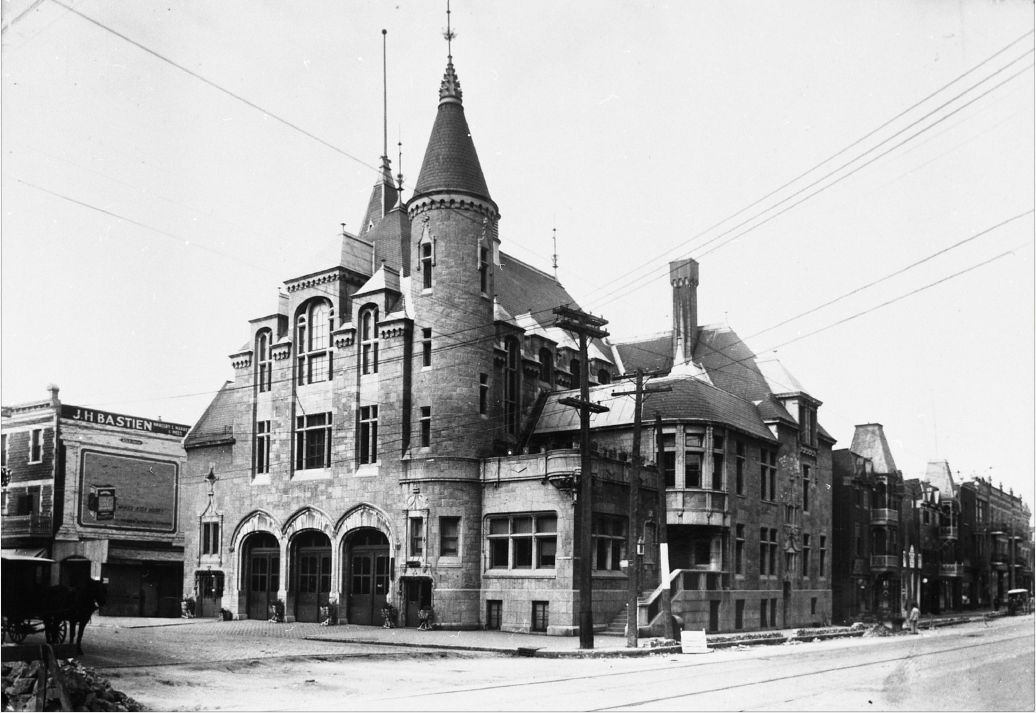
\includegraphics[width=7.7 cm]{old_montreal.png} 
\caption{\scriptsize Firemen casern in the early 1930s}
\end{figure} 


For the training, we are using modern-day pictures of the same city, which should have similar colors. However, this presents two major difficulties: first, while some objects have typical colors (snow is white, the sky is most often blue, urban roads are grey), many can have different colors: the same car could be red or blue, and have the same grayscale translation in both cases. Therefore, there is not one single "good" answer to an algorithm that gives colors to a grayscale image, rather a set of possible colors. Secondly, we use nowadays Montreal as a training set, which biases a bit the result: it is more difficult to see differences between old and modern Montreal if we color old pictures in a way that makes them look like modern Montreal: we can't really capture the changes.

\section{Related work}
Several colorizing methods have already been studied and used, for purposes of research, historic studies or documentaries for instance. We can classify them as manual, human-assisted and fully automatic methods. Manual methods cover frame-by-frame hand colorization, used for instance in re-colorization of old movies \cite{WW1Colorized}, but also computer-assisted colorization, with major softwares such as Photoshop \cite{photoshop}, that offer interesting tools for a user to add colors to a grayscale image at will. However, these methods are very costly in terms of human time spent, especially for a big number of pictures to treat (large datasets, films...), so the need for more automatic methods grew. In \cite{pap:userInput}, the authors propose an automatic method with human intervention: the algorithm uses the grayscale image and a set of pixels provided by the user to color the rest of the image: see figure \ref{fig:userInput}. 

\begin{figure}[h]
\centering
   \subfloat[\scriptsize Original image and user-provided colors]{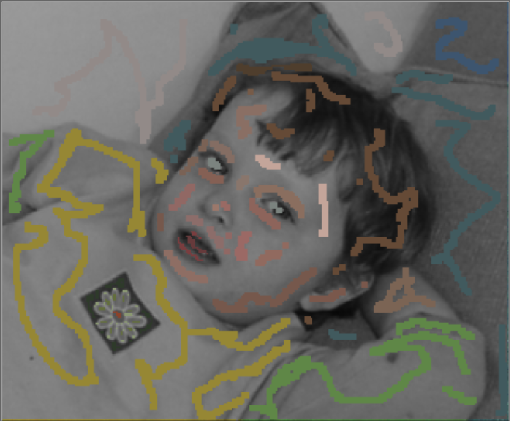
\includegraphics[width=3.5cm]{gili_m.png}}
   \subfloat[\scriptsize Result]{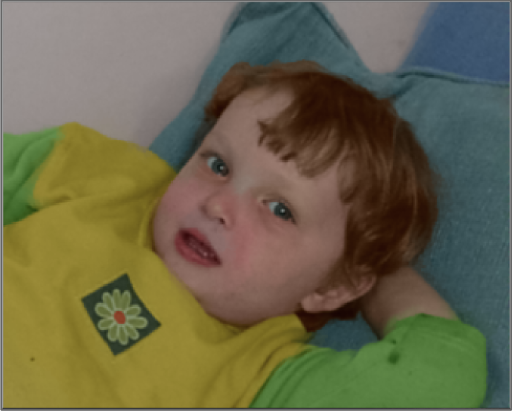
\includegraphics[width=3.5cm]{gili_res.png}}
\caption{\scriptsize Method with user input}      
\label{fig:userInput}
\end{figure}

Finally, in \cite{bestPaper}, Charpiat et al. use SURF features and SVM to predict the colors of a grayscale image by training on a similar one: see figure \ref{fig:charpiat}. Their method uses classification rather than regression, so they only get a finite number of possible colors, and most of all the user has to select an image very similar to the target for training. Our goal is to train once and for all on a large dataset of images, and then be able to color any grayscale image without having to manually pick a similar one. In \cite{stanford}, a group of students tackle the same problem with similar methods and some more computer vision-specific techniques, such as edge detection and use of graph cuts.

\begin{figure}[h]
\centering 
 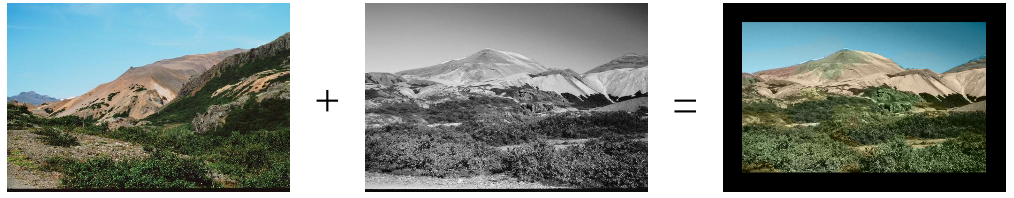
\includegraphics[width=7.7 cm]{charpiatResult.png} 
\caption{\scriptsize Result obtained by Charpiat et al. for one training and one target image}
\label{fig:charpiat}
\end{figure} 


\section{Methodology}
Learning a color mapping from a set of color images to a grayscale image cannot be done a global manner. We propose to learn a color mapping from a patch of grayscale pixels and outputting a color prediction of the middle pixel. This transforms the problem into a more feasible prediction problem by learning the color of a pixel given the grayscale content of neighboring pixels. Such an approach would inflict a reduction in the size of the image due to the inability to predict the color of pixels on the edge, however, such a loss would not reduce the image's size by a large amount.
Multiple transformations are undergone before the datasets at hand are usable:

\subsection{Resizing Images}
Input images vary greatly in terms of their size, and such variations would lead to inconsistent content of generated patches. We alter the size of images by resizing them to have a maximum dimension of 600 pixels.
L-a-b color space:
Usually a pixel color has 3 degrees of freedom, represented by the 3 channels red - blue - green (RGB). However, for each pixel that we want to color, we already know its grayscale, which removes one degree of freedom and leaving only two values to predict. To handle that, we used the L-a-b color space, which is a mapping of the RGB space, in which L is the luminance channel, so basically an equivalent of the level of gray. 

That being given, we only have to train our methods to learn values of a and b on each pixel. Then we can use the L value (that we can infer from the grayscale value of the pixel) to get the whole L-a-b value, and translate it back in RGB. 

\subsection{Generating Patches}

One of the purposes of our method is to learn from a variety of images how to color a given image. The training examples can be more or less close to the input image and therefore help color the input image with a different efficiency.
For one input image, we decided to take a bunch of recent colored images of buildings looking alike (churches in general to color the Basilique Notre Dame), at different angles and times of the day. With these images as inputs, we generate patches from each of them. For one input image of 600 pixels as max dimension, we take patches of sizes for instance 100x100 (that we will later use to predict the color of the pixel in the middle of the patch). With such an image, we would then have to compute up to $500^2$ patches of size $100 \times100$. This would have to be again multiplied by the number of images we wanted to use to train our model. For 600 pixel images, with patches of size $100 \times100$, each dataset of LAB arrays for each image would be of size around 20GB. Our first approach to reduce the size of each numpy array was to simply reduce the size of the patches but we soon realized that too small patches would mean that we would ask our convnet to predict a color with giving it too small images to be able to put them in a context. We then unfortunately had to reject this method and decided to load for an image only a small percentage of the patches: $1\%$ in our case. Indeed for most of the patches, its neighbors will contain the exact same information and using each and every possible patch in an image would mean that we do a lot of overlapping. We still had rather big files to load and this was part of one of our concern and limitation to predict colors. For instance, when we wanted to decrease our computation time using the GPU, it had only a memory of 4GB and therefore we had to keep our files on the CPU memory instead of using the usual shared function of the theano library \cite{theano1} \cite{theano2}.

A possible improvement in generating patches was to use a multi-channels CNN in order to have for the first layer, to predict the color of one pixel, 2 or 3 patches of different sizes in order to predict more efficiently and with better accuracy its color, as suggested the Recurrent Attention Model in \cite{http://arxiv.org/pdf/1406.6247v1.pdf}.

We had the idea of computing more elaborate features, such as SIFT or SURF features, instead of the patches, as done in \cite{bestPaper}. However, a convolutional neural network is supposed to be able to learn them if needed. Since we?re using it, there is no need for these features.

\subsection{CNN with regression on top}
Methods such as SVM being already tried and used, our goal was to use deep learning on the coloring problem. In particular, convolutional neural networks (CNN) seem fit for this task, since they are well suited for work on images. We used the libraries numpy \cite{numpy} (for matrix computation) and theano \cite{theano} (to use the GPU), and our own code for the CNN. 

Our goal being to predict two continuous values (for a and b), we tried to use regression first, with a convolutional network in which the last layer is a linear regression. We tried to vary the number of layers, and used up to 2 convolutional and pooling layers, and 2 hidden layers. However, the results were not good for this: see figure \ref{fig:WarholRegression}. The regression output is only gray pixels with a little bit of red in some parts of the pictures. A part of this grey being due to L-a-b values that do not exist, and correspond to no color. By rescaling properly the output, we can see that the whole picture gets colored, and that all the edges are clearly marked in the colored output. So regression can learn to put different colors on different objects, but even by changing the parameters and the scaling at the end we could never get these colors to be real-life possible ones.


\subsection{Use of clustering and classification}
Classification allowed us to have more believable color outputs, and not to get weird color and color gradients. The method with clustering the colors for the training input images and then classifying for the prediction image gave us an acceptable result that confirmed that our implementation of the convolutional neural network, which was exactly the same except for the last layer of classification instead of regression, was not in question in our previous attempts, but rather our choices of parameters in the limit of computation time and abilities that we had.

To use classification, we need to get a subset of the colors. We first used a simple regular division of the possible values for a and b, which gave bad results: an image with colors clustered that way does not look good at all. So we switched to k-means on a and b separately, with k=10. This value was chosen to have a reasonable number of classes, but a good-looking output. Figure \ref{fig:DiscretizedImage} shows the difference between a colored image and the same with clustered colors. We only cluster values for a and b, and use the initial L value in each pixel to get the complete color.

We then modified our CNN to use it for classification rather than regression. The result is shown in figure \ref{fig:result} for different numbers of clusters.

\section{Testing}
The theoretical difficulty of our task lies in the absence of obvious evaluation for the output: since a car can be red or blue, we can?t really define an error for a color put on a car, except by visual inspection. So the best error estimate is just the human perception of the image: are the colors likely or not according to the viewer? However, to train the CNN, we need to provide it an error for each color mapping. On training images, we know the real color of the objects, so we used the difference between the prediction and the actual color, measured by the mean-squared error in the case of regression, which has little meaning by itself but can be used for training, and the ratio of accuracy in the case of classification. Then, to evaluate the efficiency of our method, the best is still visual inspection of the result.

\section{Empirical results} 
We made several attempts to color the image of the Basilique Notre-Dame and our most conclusive one was using a CNN with classification and clustering of the colors of the training examples.
At first we attempted to get results using a linear regression. We obtained very precise distinction of the limits of the building and the different elements in the image but the actual output color predicted was unfortunately extremely far from anything possible. We tried with different patch sizes (10, 25), very different network complexities in terms of number of layers involved, number of Kernels, number of hidden units or pool sizes. The best output that we could get were still not close enough to the solution to be considered: see figure \ref{resultRegression}.

Then we tried to use classification on top of the CNN which would first allow us to control the range of colors that we could get for the output and we also thought we were more likely to get results from this since it were what the other papers did to try and get results. The best result we could get was done with the following parameters for the CNN:.

We can see that the result is still weak and rather far from a good colorization of the image, even with a network already complex and asking a long computation time. Fortunately we had the chance to be able to use a rather simple GPU (NVIDIA with 4GB of memory) but that could still help us reduce the computation time and try more parameters combinations.

\section{Final discussion} 
Our results, compared to the ones obtained by the papers we studied, are quite disappointing: none of our methods achieved a satisfying colorization of the grayscale images. They all seem to detect different textures in the image, and to give them different colors, but these colors do not fit at all with what we expect in real-life (they correspond more to pop-art colors). Shifting from regression to classification improves significantly the result, maybe by avoiding too high values for a and b. The convolutional neural network does not seem well adapted for inferring colors from patches, although we expected it to outperform the SURF feature + SVM used by Charpiat et alii \cite{bestPaper}.

Maybe training on several images is also still too challenging: the other authors use the colors of only one image to color another one, that has to be similar, so their methods seek a kind of overfitting on the colors of the training image. It is possible that adding data from different images perturbs this process. 

Increasing the size of the patches again, using SIFT features and using even more complex networks might be necessary to improve the result. Maybe it is also too hard to train on several images and then predict the colors in several others, maybe we have to use just one well-chosen training image for each target image. 
Would the learning part have worked better, we thought of improving the result with some kind of smoothing on the output, using a filter or rather graph cuts, to get more coherent colors. We could also have tried to reduce the effects of color discretization.

$\checkmark$ \textbf{We hereby state that all the work presented in this report is that of the authors. }

\bibliographystyle{plain}
\bibliography{report-bib.bib}
\nocite*


\end{document} 
